\section*{Conclusion}

\begin{figure*}
	\centering
	\begin{minipage}{1.5\columnwidth}
		\centering
		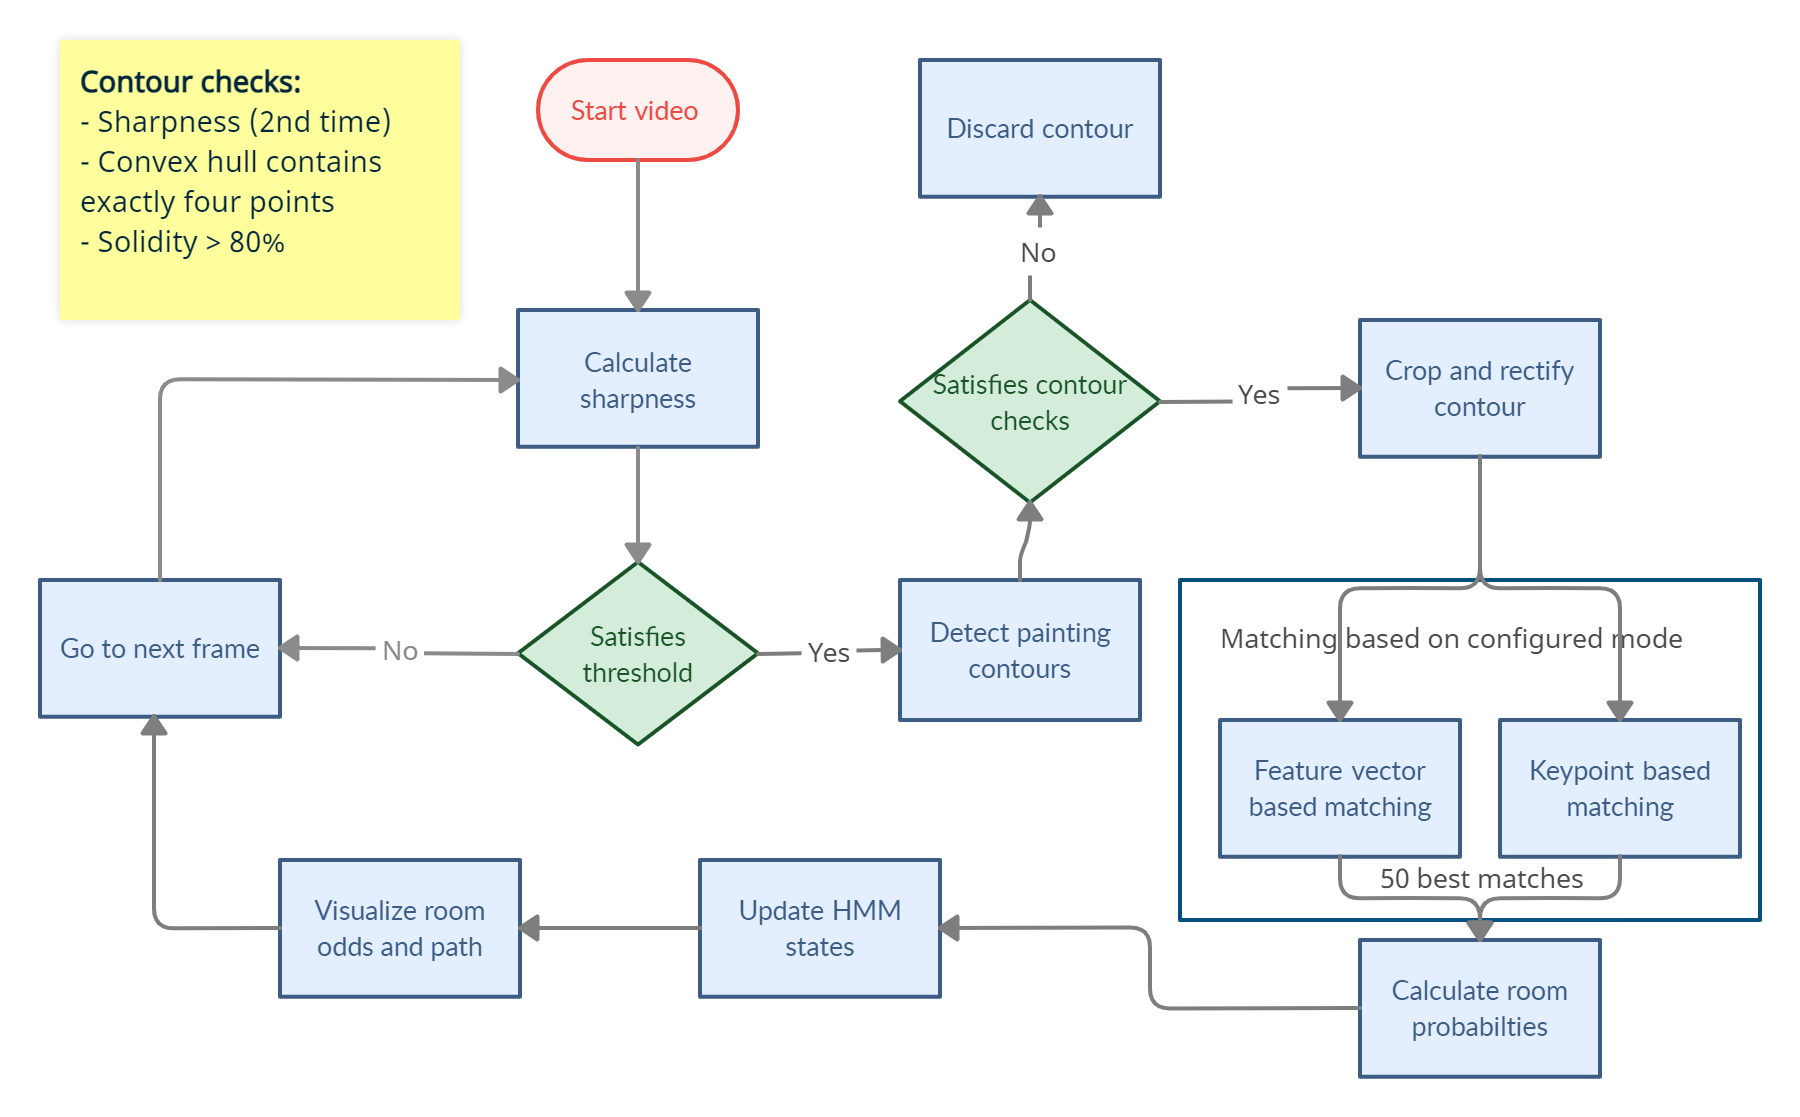
\includegraphics[width=\textwidth]{images/boxchart.png}
		\caption{Block diagram of the complete pipeline}
		\label{fig:blockdiagram}
	\end{minipage}%
\end{figure*}


% In feite wordt dit in het abstract beschreven
% Visual positioning prevents the necessity of a direct line of sight for signal transmissions or the scattering of beacons inside the building. When applied to the museum MSK Ghent it provides visitors with the number of the current room they are in. The visitors make videos of the route they take in the museum. From those videos, their location is determined. 


The final process is visualized in figure \ref{fig:blockdiagram}. The sequence of all steps ensures a working implementation.

First, the sharpness of the frame is calculated. When the sharpness is too low and doesn't satisfy the defined threshold, the frame is discarded. When the sharpness does satisfy the threshold, the frame is used to detect the painting contours. The detected painting contours are also checked. When the contours don't meet all the conditions, the frame is discarded. When the conditions are met, the painting is extracted, cropped, and rectified to get the frontal view.

After these steps, the matching itself starts. This is done with a combination of keypoint matching and feature vector matching. The best 50 matches from the database are sought. From those matches, the room probabilities (probabilities of the painting in a certain room) are calculated. The hidden Markov model then calculates the final room probabilities holding into account the location of the paintings in the previous frame. 

The predictions are then visualized with color on the floor plan of the MSK Ghent. Finally, the path most likely used by the user is also drawn on the floor plan.

When using the techniques on the videos, room for improvement can be determined (wrong matches, incorrect detections, etc.). Although remarkable good results are obtained. Next to improvements related to detection and wrong matching an optimization of the time each frame needs to compute may also be an improvement. This may be solved with multithreading. Nevertheless, the final implementation provides a good proof of concept considering various algorithms and techniques.


% In the final results, there are still some faults when running the program so there is of course still room for improvement. The program also requires a lot of processing powers. Nevertheless, it is a good working program. It can detect and match the painting's end determine the location of the user well. 

